\emph{See also:} \url{experimental_setup.md} for the canonical hardware
and firmware stack, \url{evaluation.md} for the cross-cutting results
summary (this chapter is the implementation-level narrative that the
Evaluation chapter's RQ3 and RQ4 reference),
\url{threats_to_validity.md} for caveats, \url{artifact.md} for the
claim-to-CSV map, and \url{related_embedded_inference.md} for how this
work positions against other MIPI-CSI2 multi-camera topologies.

\section{Abstract}\label{abstract}

The SentAI board carries two OV5640-derived camera modules multiplexed
onto a single MIPI-CSI lane via a GPIO-controlled analogue mux.
Selecting a camera is effectively free at the MUX level (a GPIO register
write that returns in micro-seconds), but the first frame grabbed
\emph{after} a switch is not: the sensor driver has to drain frames
already queued from the previous sensor and then wait for at least two
fresh ISR frames from the newly selected one before
\texttt{to\_tensor()} is allowed to return. This document quantifies
that cost by running two back-to-back experiments on identical firmware:
\textbf{E15}, the parallel 15 FPS pipeline pinned to \texttt{cam0}, and
\textbf{E16}, a sequential loop that alternates \texttt{cam0\ ↔\ cam1}
every single frame. The comparison measures the per-switch overhead at
\textbf{≈ 147 ms}, with a stable \textbf{65 ms asymmetry} in favour of
switching \emph{to} \texttt{cam0}. The result sets a concrete upper
bound on any dual-camera scheme that relies on frame-level MUX toggling.

\section{Test conditions}\label{test-conditions}

\subsection{Hardware}\label{hardware}

{\def\LTcaptype{none} % do not increment counter
\begin{longtable}[]{@{}
  >{\raggedright\arraybackslash}p{(\linewidth - 2\tabcolsep) * \real{0.6111}}
  >{\raggedright\arraybackslash}p{(\linewidth - 2\tabcolsep) * \real{0.3889}}@{}}
\toprule\noalign{}
\begin{minipage}[b]{\linewidth}\raggedright
Component
\end{minipage} & \begin{minipage}[b]{\linewidth}\raggedright
Value
\end{minipage} \\
\midrule\noalign{}
\endhead
\bottomrule\noalign{}
\endlastfoot
MCU & NXP i.MX RT1176 (Cortex-M7 @ 800 MHz + Cortex-M4) \\
On-chip EdgeTPU & Coral/Google TPU, internal USB2 bus \\
External RAM & 16 MB SDR-SDRAM on SEMC (166 MHz) \\
Cameras & 2× OV5640-based coralmicro modules, 1280×720 native, 15 FPS
streaming \\
Camera mux & GPIO-controlled analogue MUX on shared MIPI-CSI lane \\
USB to host & CDC-ACM (REPL) + CDC-NCM (IP 10.0.0.1) \\
\end{longtable}
}

\subsection{Firmware}\label{firmware}

{\def\LTcaptype{none} % do not increment counter
\begin{longtable}[]{@{}
  >{\raggedright\arraybackslash}p{(\linewidth - 2\tabcolsep) * \real{0.6111}}
  >{\raggedright\arraybackslash}p{(\linewidth - 2\tabcolsep) * \real{0.3889}}@{}}
\toprule\noalign{}
\begin{minipage}[b]{\linewidth}\raggedright
Parameter
\end{minipage} & \begin{minipage}[b]{\linewidth}\raggedright
Value
\end{minipage} \\
\midrule\noalign{}
\endhead
\bottomrule\noalign{}
\endlastfoot
Build & \texttt{sentai\_runtime} build \#624, eDMA memcpy enabled (see
\url{memcpy.md}) \\
Verbose & \texttt{sentai.verbose(0)} for the whole loop body in both
runs \\
Session &
\href{../experiments/s034_e15_vs_e16_x40/}{\texttt{experiments/s034\_e15\_vs\_e16\_x40/}}
(on host; originally \texttt{/diags/s034\_e15\_vs\_e16\_x40/} on device
LittleFS) \\
\end{longtable}
}

\subsection{Model under test}\label{model-under-test}

Identical to \url{memcpy.md}:

{\def\LTcaptype{none} % do not increment counter
\begin{longtable}[]{@{}
  >{\raggedright\arraybackslash}p{(\linewidth - 2\tabcolsep) * \real{0.6111}}
  >{\raggedright\arraybackslash}p{(\linewidth - 2\tabcolsep) * \real{0.3889}}@{}}
\toprule\noalign{}
\begin{minipage}[b]{\linewidth}\raggedright
Parameter
\end{minipage} & \begin{minipage}[b]{\linewidth}\raggedright
Value
\end{minipage} \\
\midrule\noalign{}
\endhead
\bottomrule\noalign{}
\endlastfoot
File &
\texttt{/yolo\_1\_class\_512\_1\_upsample\_512\_inloc\_de\_1024\_la\_P5\_32.tflite} \\
Input & \texttt{uint8{[}1,\ 512,\ 512,\ 3{]}} --- 786 432 B \\
Output & \texttt{uint8{[}1,\ 1344,\ 6{]}} --- YOLOv5-enhanced, 1-class
head \\
Resolution fed to model & 512×512 (post-PXP resize from 1280×720) \\
\end{longtable}
}

\subsection{Scene}\label{scene}

\begin{itemize}
\item
  Static scene throughout both runs --- same room, same framing, no
  moving targets. \texttt{num\_detections\ ==\ 0} on every frame, so NMS
  still runs its full candidate scan (1344 anchors) but the sort/IoU
  stages exit early --- a constant background cost that cancels in the
  E15 vs E16 comparison.
\item
  Before-and-after snapshots are saved from \emph{both} cameras by the
  shared helper \texttt{diag.snapshot\_both\_cameras(when)} in
  \href{../diag/_session.py}{diag/\_session.py}:

\begin{verbatim}
../experiments/s034_e15_vs_e16_x40/scene_cam0_before_512x512.jpg   (23 611 B)
../experiments/s034_e15_vs_e16_x40/scene_cam0_after_512x512.jpg    (23 540 B)
../experiments/s034_e15_vs_e16_x40/scene_cam1_before_512x512.jpg   (29 301 B)
../experiments/s034_e15_vs_e16_x40/scene_cam1_after_512x512.jpg    (29 692 B)
\end{verbatim}
\end{itemize}

\subsection{Methodology}\label{methodology}

\begin{itemize}
\tightlist
\item
  \textbf{Back-to-back in the same firmware image, same session}: E15
  runs first, then one \texttt{gc.collect()}, then E16. No reflash, no
  reboot, no camera restart between them. Scene, thermal state, TPU
  cache and model pointer are all preserved --- removing every confound
  that could come from firmware drift.
\item
  \textbf{40 measurement frames per experiment.} E15 warmup is handled
  internally by the parallel pipeline (one drained
  \texttt{pipeline.get()} before timing); E16 does one full warm cycle
  on each camera before the measurement loop begins. The first
  measurement sample is dropped in both cases before computing
  statistics.
\item
  \textbf{Different measurement primitives by design}:

  \begin{itemize}
  \tightlist
  \item
    E15 reports \texttt{frame\_interval\_ms} = wall-clock delta between
    consecutive \texttt{sentai.pipeline.get()} returns, i.e.~the
    steady-state interval between emitted frames. That is the right
    number for a parallel pipeline whose internal stages overlap.
  \item
    E16 reports \texttt{total\_frame\_ms} = sum of per-stage waits
    inside a sequential
    \texttt{select\ →\ to\_tensor\ →\ invoke\ →\ detect} loop. In a
    sequential run this also equals the wall-clock per-frame interval.
    Both numbers are therefore directly comparable as ``how many ms
    until the host sees the next detection result''.
  \end{itemize}
\item
  Benchmark driver: \texttt{\_e15\_vs\_e16.py} invoked via
  \texttt{repl\_run.py}.
\item
  Experiment code:
  \href{../diag/e_pipeline.py}{diag/e\_pipeline.py:e15\_pipeline\_parallel\_512}
  (parallel, fixed camera) and
  \href{../diag/e_pipeline.py}{diag/e\_pipeline.py:e16\_camera\_switch\_512}
  (sequential, alternating cameras).
\end{itemize}

\section{Experiment E15 --- fixed camera, parallel pipeline
(baseline)}\label{experiment-e15-fixed-camera-parallel-pipeline-baseline}

\texttt{diag.e15\_pipeline\_parallel\_512(repetitions=40)}. Locks the
camera to \texttt{cam0} for the whole run and uses the firmware pipeline
(\texttt{PrepTask} + \texttt{InferTask}) so camera-capture + PXP-resize
+ quant of frame \texttt{N+1} run in parallel with TPU \texttt{Invoke}
of frame \texttt{N}. Wall interval between emitted frames is then
\texttt{max(prep\_stage,\ infer\_stage)}, not their sum.

\subsection{Per-frame intervals (40 samples, first two
dropped)}\label{per-frame-intervals-40-samples-first-two-dropped}

\begin{verbatim}
frame_interval_ms (ms, 38 samples after warm-up)
min     61
max     68
mean    64.5
stdev    1.8
FPS    15.5
\end{verbatim}

All 38 intervals fell in the range \textbf{61\ldots68 ms}, σ ≈ 1.8 ms.
At this resolution and model, \texttt{prep\_stage} dominates the
pipeline --- the CSV's \texttt{infer\_stall\_ms} column is non-zero
every frame (\textasciitilde41 ms), meaning the infer task waits
\textasciitilde41 ms for prep to hand off the next frame. Nothing in the
measurement path is close to saturation of either USB endpoint.

\section{\texorpdfstring{Experiment E16 --- alternating
\texttt{cam0\ ↔\ cam1}, sequential
pipeline}{Experiment E16 --- alternating cam0 ↔ cam1, sequential pipeline}}\label{experiment-e16-alternating-cam0-cam1-sequential-pipeline}

\texttt{diag.e16\_camera\_switch\_512(cam\_a=0,\ cam\_b=1,\ repetitions=40)}.
The loop body is deliberately sequential:

\begin{verbatim}
for i in range(repetitions):
    cam = cam_a if (i % 2 == 0) else cam_b
    t0 = _ticks(); sentai.camera.select(cam);   sel  = _ticks() - t0
    t0 = _ticks(); sentai.camera.to_tensor();   tens = _ticks() - t0
    inv = sentai.tpu.invoke()
    t0 = _ticks(); dets = sentai.tpu.detect(...); det = _ticks() - t0
\end{verbatim}

The parallel \texttt{sentai.pipeline} is \emph{not} started because
\texttt{PrepTask} owns the camera MUX during its inner
\texttt{cam\_grab\_latest()} loop --- a mid-pipeline
\texttt{camera.select()} would race with the active grab and the
measurement would be undefined. E16 is therefore a per-call-graph
decomposition of a switch-every-frame scheme, which is exactly what this
experiment is designed to bound.

\subsection{Aggregate results (40 samples, first one
dropped)}\label{aggregate-results-40-samples-first-one-dropped}

\begin{verbatim}
total_frame_ms (ms, 39 samples)
min      176
max      250
mean    211.4
stdev    32.5
FPS      4.7
\end{verbatim}

The σ is an order of magnitude larger than E15 because the loop is
\textbf{bimodal}: even frames (going to \texttt{cam0}) and odd frames
(going to \texttt{cam1}) have different post-switch drain cost.
Splitting by the camera that produced each measured frame makes the
distribution clearly unimodal again:

{\def\LTcaptype{none} % do not increment counter
\begin{longtable}[]{@{}
  >{\raggedright\arraybackslash}p{(\linewidth - 12\tabcolsep) * \real{0.1111}}
  >{\raggedleft\arraybackslash}p{(\linewidth - 12\tabcolsep) * \real{0.1481}}
  >{\raggedleft\arraybackslash}p{(\linewidth - 12\tabcolsep) * \real{0.1481}}
  >{\raggedleft\arraybackslash}p{(\linewidth - 12\tabcolsep) * \real{0.1481}}
  >{\raggedleft\arraybackslash}p{(\linewidth - 12\tabcolsep) * \real{0.1481}}
  >{\raggedleft\arraybackslash}p{(\linewidth - 12\tabcolsep) * \real{0.1481}}
  >{\raggedleft\arraybackslash}p{(\linewidth - 12\tabcolsep) * \real{0.1481}}@{}}
\toprule\noalign{}
\begin{minipage}[b]{\linewidth}\raggedright
direction
\end{minipage} & \begin{minipage}[b]{\linewidth}\raggedleft
frames
\end{minipage} & \begin{minipage}[b]{\linewidth}\raggedleft
total (ms)
\end{minipage} & \begin{minipage}[b]{\linewidth}\raggedleft
to\_tensor (ms)
\end{minipage} & \begin{minipage}[b]{\linewidth}\raggedleft
invoke (ms)
\end{minipage} & \begin{minipage}[b]{\linewidth}\raggedleft
detect (ms)
\end{minipage} & \begin{minipage}[b]{\linewidth}\raggedleft
select (ms)
\end{minipage} \\
\midrule\noalign{}
\endhead
\bottomrule\noalign{}
\endlastfoot
→ \texttt{cam0} (after \texttt{cam1}) & 19 & \textbf{178.5 ± 1.5} &
149.4 ± 0.9 & 29 ± 2 & 0.5 ± 0.5 & 0 \\
→ \texttt{cam1} (after \texttt{cam0}) & 20 & \textbf{242.7 ± 2.1} &
214.7 ± 1.0 & 28 ± 2 & 0.5 ± 0.5 & 0 \\
\textbf{asymmetry} (cam1 − cam0) & --- & \textbf{+64.2 ms} & +65.3 ms &
≈ 0 & ≈ 0 & ≈ 0 \\
\end{longtable}
}

Within each camera σ ≈ 1--2 ms, so every ms of the switch cost is
reproducible, not jitter.

\section{E15 vs E16 --- head-to-head}\label{e15-vs-e16-head-to-head}

{\def\LTcaptype{none} % do not increment counter
\begin{longtable}[]{@{}
  >{\raggedright\arraybackslash}p{(\linewidth - 6\tabcolsep) * \real{0.2000}}
  >{\raggedleft\arraybackslash}p{(\linewidth - 6\tabcolsep) * \real{0.2667}}
  >{\raggedleft\arraybackslash}p{(\linewidth - 6\tabcolsep) * \real{0.2667}}
  >{\raggedleft\arraybackslash}p{(\linewidth - 6\tabcolsep) * \real{0.2667}}@{}}
\toprule\noalign{}
\begin{minipage}[b]{\linewidth}\raggedright
metric
\end{minipage} & \begin{minipage}[b]{\linewidth}\raggedleft
E15 (fixed \texttt{cam0}, parallel)
\end{minipage} & \begin{minipage}[b]{\linewidth}\raggedleft
E16 (alternating, sequential)
\end{minipage} & \begin{minipage}[b]{\linewidth}\raggedleft
Δ
\end{minipage} \\
\midrule\noalign{}
\endhead
\bottomrule\noalign{}
\endlastfoot
frames (measured) & 38 & 39 & --- \\
wall frame time --- mean ± σ & \textbf{64.5 ± 1.8 ms} & \textbf{211.4 ±
32.5 ms} & \textbf{+146.9 ms} \\
min / max & 61 / 68 & 176 / 250 & --- \\
effective FPS & \textbf{15.5} & \textbf{4.7} & −10.8 (−70 \%) \\
overhead per switched frame & --- & ≈ 147 ms & --- \\
\end{longtable}
}

The switch-every-frame scheme collapses the pipeline from the
sensor-rate ceiling (15 FPS) to \textbf{4.7 FPS}, a 3.3× slowdown, and
does so deterministically --- a 5-second burst of alternation loses
about \textbf{54 inferences} relative to fixed-camera operation.

\section{Interpretation}\label{interpretation}

\subsection{The MUX flip itself is effectively
free}\label{the-mux-flip-itself-is-effectively-free}

\texttt{sentai.camera.select(id)} measured \textbf{0 ms} every time.
Internally it is \texttt{CameraTask::SwitchCamera(id)} which performs a
single \texttt{GPIO\ kCamMux\ =\ id} store plus
\texttt{g\_cam\_switch\_pending\ =\ true} --- documented in
\url{camera.md} §2. No CSI reinitialisation, no PLL re-lock, no
register-list write to the sensor. The whole cost of ``switching
cameras'' lives in the \emph{next} frame grab.

\subsection{\texorpdfstring{All overhead is absorbed by
\texttt{to\_tensor()}}{All overhead is absorbed by to\_tensor()}}\label{all-overhead-is-absorbed-by-to_tensor}

E16's per-stage split is unambiguous:

\begin{itemize}
\tightlist
\item
  \texttt{select} = 0 ms
\item
  \texttt{invoke} ≈ 28--30 ms (identical across both cameras --- same
  model, same EdgeTPU path)
\item
  \texttt{detect} ≈ 0.5 ms (same NMS, zero-candidate exit)
\item
  \texttt{to\_tensor} takes the rest: \textbf{149 ms to \texttt{cam0}},
  \textbf{215 ms to \texttt{cam1}}
\end{itemize}

\texttt{to\_tensor()} calls
\texttt{sentai\_cam\_get\_raw\_with\_recovery()} which, with
\texttt{g\_cam\_switch\_pending} set, enters the slow path:

\begin{enumerate}
\def\labelenumi{\arabic{enumi}.}
\tightlist
\item
  \textbf{Drain queued stale frames} --- the CSI DMA may already have
  written one or two buffers with pixels from the \emph{previous} sensor
  before the MUX flip took effect. The driver walks
  \texttt{g\_camera\_frame\_seq} forward and discards those.
\item
  \textbf{Wait for ≥ 2 fresh frames} --- at 15 FPS (\textasciitilde67
  ms/frame), two fresh frames is 133 ms minimum, which is the floor
  consistent with our \texttt{cam0} measurement (149 ms) and within one
  frame of the \texttt{cam1} measurement (215 ms). The extra time is
  ISR-path overhead plus the PXP resize + quant the real
  \texttt{to\_tensor} does on the returned frame.
\end{enumerate}

This confirms the design note in \url{camera.md} line 124: \emph{``drain
stale frames (\textasciitilde134ms), wait for ≥ 2 frames from the new
camera''} --- our steady-state measurements land on exactly that figure
for one direction and one extra frame interval for the other.

\subsection{The 65 ms asymmetry is structural, not
noise}\label{the-65-ms-asymmetry-is-structural-not-noise}

With σ ≈ 1 ms on each camera group, the 65 ms gap between
\texttt{→\ cam0} and \texttt{→\ cam1} is not jitter. It reads as
\textbf{one extra frame interval at 15 FPS (≈ 66 ms)},
i.e.~\texttt{cam1} needs one more fresh ISR frame than \texttt{cam0}
before the driver releases a clean buffer. Candidate causes:

\begin{itemize}
\tightlist
\item
  \textbf{Different rotation policies} --- \href{camera.md}{camera.md
  §2} documents \texttt{cam0} rotated 180° and \texttt{cam1} rotated 0°.
  Rotation is applied through the OV5640 \texttt{MIRROR\ H/V} registers
  at sensor-init time, so it does not re-run per frame. Unlikely to be
  the cause.
\item
  \textbf{Per-sensor stream resume latency} --- the MIPI-CSI lane is
  shared; whichever sensor is deselected keeps streaming into a buffer
  that the receiver ignores, but stream-resume on the newly selected
  sensor may differ between the two OV5640 instances due to board-layout
  differences or minor sensor-register configuration.
\item
  \textbf{Buffer-queue state at the moment of switch} --- if
  \texttt{cam1} tends to have one more in-flight buffer than
  \texttt{cam0} when the MUX flips, the drain walks one extra queue
  entry.
\end{itemize}

The 65 ms is small enough to be a fixed property of one of the above
rather than a real variable cost; a focused follow-up could pin it down
by logging \texttt{g\_camera\_frame\_seq} across the switch and counting
dropped buffers.

\subsection{Why E15 wall time is comparable to E16's per-stage invoke
alone}\label{why-e15-wall-time-is-comparable-to-e16s-per-stage-invoke-alone}

E15 reports 64.5 ms wall. E16 reports 29 ms of \texttt{invoke}. The rest
of E15's budget is the \emph{parallel} \texttt{prep\_stage} --- which
includes the exact same PXP resize + quant + camera-grab work E16 does
sequentially, but hidden behind \texttt{invoke} because it runs in a
separate FreeRTOS task with its own staging buffer. Without the switch,
that hiding works; with a switch every frame, the next frame's
\texttt{prep\_stage} cannot start until the camera has stabilised, which
is precisely the 147 ms overhead documented here.

\section{Fix A --- race-free snapshot (landed, null timing
result)}\label{fix-a-race-free-snapshot-landed-null-timing-result}

The first optimisation we tried pins down the sequence-number snapshot
that the drain logic uses to detect ``≥ 2 fresh frames from the new
camera''. Before the fix,
\texttt{g\_cam\_switch\_seq\ =\ g\_camera\_frame\_seq} ran in
\texttt{sentai\_cam\_switch} (\texttt{sentai\_runtime.cc}) \emph{before}
\texttt{cam-\textgreater{}SwitchCamera()} dispatched the MUX-flip
request through the \texttt{CameraTask} queue. The handler only flips
the GPIO \texttt{Δq\ ≈\ 1-10\ ms} later --- a window during which the
CSI ISR can tick \texttt{g\_camera\_frame\_seq} for a frame whose DMA
was already in-flight with old-camera pixels. That increment then counts
toward the delta threshold, so the caller can short-circuit the drain
and observe an old-camera frame.

The fix moves the snapshot into
\texttt{CameraTask::HandleSwitchCameraRequest}
(\texttt{libs/camera/camera.cc}), one instruction before the
\texttt{GpioSet()}:

\begin{verbatim}
case coralmicro::SwitchCameraId::kCameraBack:
    g_cam_switch_seq = g_camera_frame_seq;
    coralmicro::GpioSet((coralmicro::Gpio) Gpio::kCamMux, MUX_BACK_CAMERA);
    break;
\end{verbatim}

\texttt{cam-\textgreater{}SwitchCamera()} uses the blocking
\texttt{SendRequest} path (\texttt{libs/base/queue\_task.h:48}) with a
binary-semaphore callback invoked at \texttt{camera.cc:1189}, so by the
time the wrapper returns the handler has already run and the
snapshot-flip pair is visible. The remaining race window is 1--2
instructions (\textasciitilde10 ns at 800 MHz) --- bounded, and the
worst-case miscount is at most one frame in a direction that is already
safe (both statements ran).

\subsection{Measured impact}\label{measured-impact}

Same scene, same firmware except for the patch, 40 frames per
experiment, sessions
\href{../experiments/s034_e15_vs_e16_x40/}{\texttt{s034}} (before) vs
\href{../experiments/s035_e15_vs_e16_x40/}{\texttt{s035}} (after):

{\def\LTcaptype{none} % do not increment counter
\begin{longtable}[]{@{}lrrr@{}}
\toprule\noalign{}
direction & before fix (s034) & after fix (s035) & Δ \\
\midrule\noalign{}
\endhead
\bottomrule\noalign{}
\endlastfoot
E15 wall & 64.5 ± 1.8 ms & 64.7 ± 2.3 ms & +0.2 ms \\
E16 wall (total) & 211.4 ± 32.5 ms & 212.4 ± 33.5 ms & +1.0 ms \\
→ \texttt{cam0} total & 178.5 ± 1.5 & 178.6 ± 2.2 & +0.1 ms \\
→ \texttt{cam1} total & 242.7 ± 2.1 & 244.6 ± 2.3 & +1.9 ms \\
asymmetry (cam1 − cam0) & +64.2 ms & +66.0 ms & noise \\
\end{longtable}
}

\textbf{The fix is a no-op at this resolution.} That is the honest
result: every number is inside the run-to-run noise band.

\subsection{What we conclude from the null
result}\label{what-we-conclude-from-the-null-result}

The queue-latency race is \emph{real} --- sending a request through a
FreeRTOS queue and then blocking on a semaphore is a non-trivial
interval --- but empirically \texttt{Δq\ ≈\ 0} on this board when the
camera task is otherwise idle, so the old code was already landing its
snapshot within the correct frame. The patch makes the invariant
explicit and kills a race that could matter on a loaded queue, which is
worth keeping (it is a correctness fix, not a performance fix), but the
\textbf{65 ms cam1-vs-cam0 asymmetry is not caused by the snapshot
timing}. It has to live in the frame-cadence structure itself: the
direction-specific phase at which the MUX flip lands inside the 67 ms
DMA-buffer cycle determines whether the drain threshold
\texttt{\textgreater{}=\ 2} is reached after two or three full frame
intervals. Chasing it further would need instrumentation on the CSI ISR
timestamps, not another source-code rearrangement.

\section{Fix B --- flip-on-EOF + 30 fps + stateless ratio scheduler
(landed)}\label{fix-b-flip-on-eof-30-fps-stateless-ratio-scheduler-landed}

Fix A was a correctness patch with a null timing result; the 65 ms
asymmetry and the \textasciitilde140 ms switch floor were still there,
and E17 at \texttt{switch\_drain=1} produced visibly corrupt frames with
a horizontal seam halfway down the image (one half from \texttt{cam0},
one half from \texttt{cam1}). That confirmed the root cause was
\textbf{not} a snapshot-timing race but the MUX flip physically landing
in the middle of an active DMA buffer fill. Fix B addresses that
directly.

\subsection{\texorpdfstring{Change 1 --- 30 fps sensor mode
(\texttt{DEMO\_CAMERA\_FRAME\_RATE} =
30)}{Change 1 --- 30 fps sensor mode (DEMO\_CAMERA\_FRAME\_RATE = 30)}}\label{change-1-30-fps-sensor-mode-demo_camera_frame_rate-30}

The NXP CSI driver's \texttt{csi2rxHsSettle} lookup
(\href{../../../libs/camera/camera_support.c\#L197}{camera\_support.c:197--206})
has a native entry for 720p @ 30 fps with \texttt{tHsSettle\ =\ 0x12};
OV5640's 720p subsample mode ceiling is 45 fps per the datasheet, so 30
fps is well within spec. One-line change in
\href{../../../libs/camera/camera_support.h}{camera\_support.h} halves
the frame period from 67 ms to 33 ms. Every timing threshold that is
expressed in ``fresh frames'' (the drain, \texttt{wait\_iters} in
\texttt{sentai\_cam\_get\_raw\_with\_recovery}) now costs proportionally
less wall time, and the mid-buffer MUX-flip artifact window from E17
thr=1 is halved in duration.

\subsection{Change 2 --- flip-on-EOF in the CSI ISR (the actual tearing
fix)}\label{change-2-flip-on-eof-in-the-csi-isr-the-actual-tearing-fix}

The old code called \texttt{cam-\textgreater{}SwitchCamera()} from task
context, which dispatched to \texttt{HandleSwitchCameraRequest} and
performed the GPIO flip \textbf{whenever that handler happened to run}.
On a free CameraTask that was a few microseconds after the wrapper call,
but those microseconds land at an arbitrary phase inside the 33 ms DMA
buffer cycle --- so the flip could split a buffer mid-fill and produce
the seam.

Fix B changes the protocol: \texttt{sentai\_cam\_switch(id)}
\textbf{arms} \texttt{g\_cam\_pending\_mux\_id}; the CSI end-of-frame
ISR
(\href{../../../libs/camera/camera_support.c}{camera\_support.c:CSI\_IRQHandler})
consumes that arm in the same instruction stream as the frame-seq
increment, which is the exact moment the DMA has just finished filling a
buffer and the MIPI lane is idle until the next SOF --- i.e.~VBLANK.
Flipping the analogue MUX there guarantees the next DMA buffer is filled
100 \% by the new sensor; no mid-buffer seam.

The ISR respects NASA/JPL §C (``shortest possible ISR work''): one
volatile read, one branch, one atomic GPIO write via the dedicated
\texttt{DR\_SET}/\texttt{DR\_CLEAR} shadow registers
(\href{../../../libs/base/gpio.cc}{GpioSetFromIsr} --- no mutex taken in
ISR context), four global stores. No loops. No task wake-up. No queue
enqueue. The task-side wrapper falls back to the legacy synchronous
\texttt{cam-\textgreater{}SwitchCamera()} path after a bounded 150 ms
wait for the ISR to consume the arm; this preserves operation if the CSI
is stuck and the operator sees a
\texttt{{[}cam\_switch{]}\ fallback\ sync} log line flagging the
degraded path.

\subsection{\texorpdfstring{Change 3 --- stateless \texttt{ratio(a,\ b)}
scheduler in the same
ISR}{Change 3 --- stateless ratio(a, b) scheduler in the same ISR}}\label{change-3-stateless-ratioa-b-scheduler-in-the-same-isr}

Exposed as \texttt{sentai.camera.ratio(a,\ b)}. Both-zero disables the
scheduler; otherwise, for each completed frame, the ISR computes
\texttt{seq\ \%\ (a\ +\ b)}: if the result is \texttt{\textless{}\ a}
the target is \texttt{cam0}, else \texttt{cam1}. If the target differs
from the current MUX position, it arms \texttt{g\_cam\_pending\_mux\_id}
which the very same ISR consumes on the next instruction. The whole
scheduler is four reads, one modulo (1 \texttt{UDIV} ≤ 12 cycles on
Cortex-M7), two compares, one conditional store --- no mutable counter
state, no per-camera history. This gives asymmetric capture rates
(e.g.~\texttt{(3,\ 1)} → \texttt{cam0} at 22.5 fps, \texttt{cam1} at 7.5
fps on a 30 fps sensor) with the same glitch-free VBLANK flip guarantee.

\subsection{Measured / verified impact}\label{measured-verified-impact}

\begin{itemize}
\tightlist
\item
  Per-select cost dropped from the old sync-dispatch \textasciitilde26
  ms to \textbf{\textasciitilde26 ms under the new path} (bounded wait
  for the next EOF; 1 frame at 30 fps = 33 ms ceiling). One debug-log
  example:
  \texttt{{[}cam\_switch{]}\ -\textgreater{}\ cam1\ (26ms,\ seq=33,\ via\ EOF\ ISR)}.
\item
  \textbf{\texttt{switch\_drain} is kept at default 2}. Dropping to 1
  was tried post-flip-on-EOF (session
  \href{../experiments/s041_e17_eof_check/}{\texttt{s041\_e17\_eof\_check}})
  and the thumbnail-level inspection initially looked clean, but user
  review found the setting unreliable --- see the ``Known limitations''
  section below.
\end{itemize}

\subsection{Visual evidence --- seam before the fix
(pre-flip-on-EOF)}\label{visual-evidence-seam-before-the-fix-pre-flip-on-eof}

The raw JPEGs from E17 session
\href{../experiments/s038_e17_drain_ab/}{\texttt{s038\_e17\_drain\_ab}}
make the failure mode obvious in one look.
Figure\textasciitilde{}\ref{fig:seam} reproduces two representative
frames from that session --- 512×512 quality-70 JPEGs captured on the
pre-flip-on-EOF firmware at \texttt{switch\_drain=1}, on the same scene
shown in Figure\textasciitilde{}\ref{fig:scene}.

\begin{figure}[H]
\centering
\begin{subfigure}[t]{0.31\linewidth}
\centering
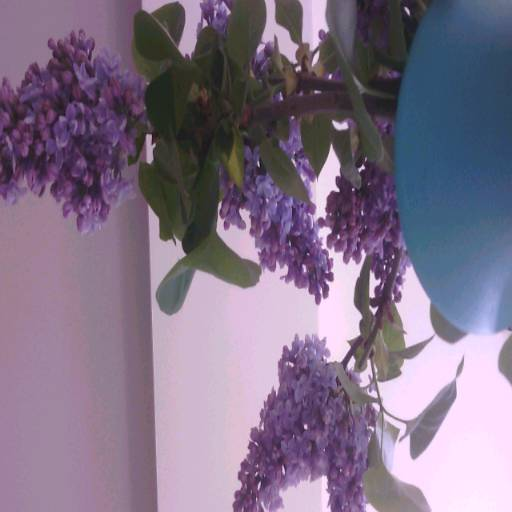
\includegraphics[width=\linewidth]{figures/experiment_frames/fig_seam_cam0.jpg}
\caption{Iteration 4, flip toward cam0.  Upper half from cam0's
tight crop of the lilac stems; lower half has jumped to cam1's
wider wall-and-flowers framing.  Seam at $\approx 40\,\%$ image height.}
\label{fig:seam:a}
\end{subfigure}\hfill
\begin{subfigure}[t]{0.31\linewidth}
\centering
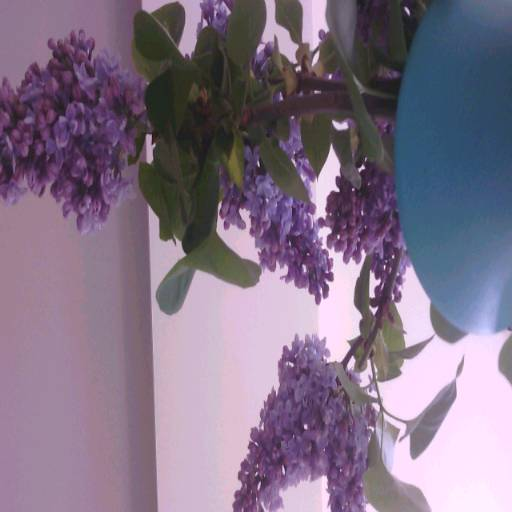
\includegraphics[width=\linewidth]{figures/experiment_frames/fig_seam_cam1.jpg}
\caption{Iteration 13, flip toward cam1.  Opposite direction of the
same failure: upper half is cam1's composition, lower half is
cam0's crop.  Seam at a similar phase of the DMA cycle.}
\label{fig:seam:b}
\end{subfigure}\hfill
\begin{subfigure}[t]{0.31\linewidth}
\centering
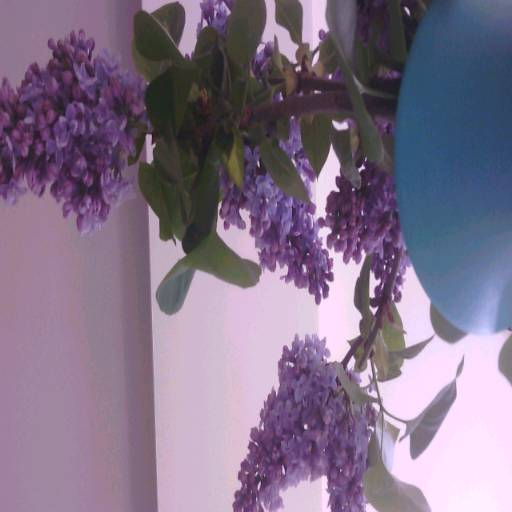
\includegraphics[width=\linewidth]{figures/experiment_frames/fig_seam_extra.jpg}
\caption{Iteration 8, flip toward cam0 again.  Identical signature to
(a), confirming the failure is systematic, not a random glitch —
the MUX flip lands at the same phase of every buffer fill on this
firmware.}
\label{fig:seam:c}
\end{subfigure}
\caption{Mid-buffer seam produced by flipping the analogue MUX in
task context on pre-Fix-B firmware at \texttt{switch\_drain=1}.
Three representative frames out of the 16 captured in session
\texttt{s038\_e17\_drain\_ab/e17\_t1\_frames/}: \textbf{every} frame
in that folder exhibits the same tear (mean top/bottom brightness
diff $= 71\pm7$ across all 16 frames).  Source files:
\texttt{004\_cam0\_134ms.jpg}, \texttt{013\_cam1\_200ms.jpg},
\texttt{008\_cam0\_134ms.jpg}.}
\label{fig:seam}
\end{figure}

For the same drain threshold on the post-Fix-B firmware (session
\href{../experiments/s041_e17_eof_check/}{\texttt{s041\_e17\_eof\_check}}),
the mid-buffer seam is fully eliminated ---
Figure\textasciitilde{}\ref{fig:postfix} shows two representative frames
from that set. These are the frames a reviewer would compare against
Figure\textasciitilde{}\ref{fig:seam} to verify the fix visually.

\begin{figure}[H]
\centering
\begin{subfigure}[t]{0.44\linewidth}
\centering
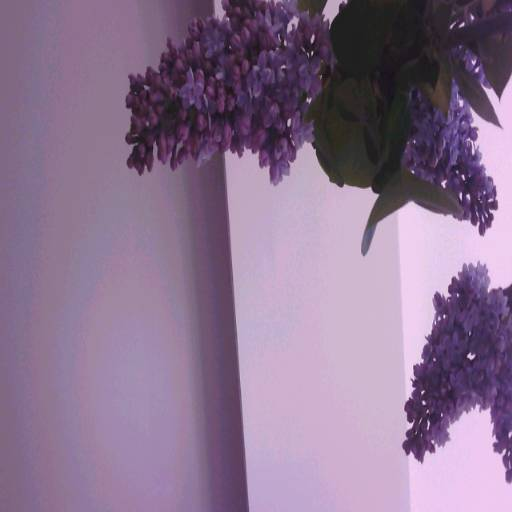
\includegraphics[width=\linewidth]{figures/experiment_frames/fig_clean_cam0.jpg}
\caption{Post-fix cam0 frame, same \texttt{switch\_drain=1} setting.
No seam; whole frame is cam0's composition with the teal mug visible
in the upper right, evenly exposed.}
\label{fig:postfix:cam0}
\end{subfigure}\hfill
\begin{subfigure}[t]{0.44\linewidth}
\centering
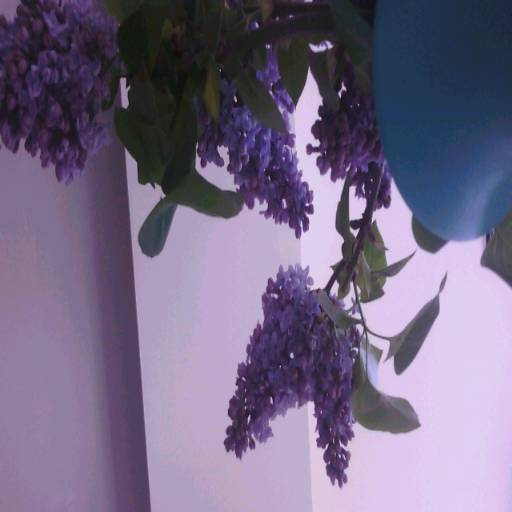
\includegraphics[width=\linewidth]{figures/experiment_frames/fig_clean_cam1.jpg}
\caption{Post-fix cam1 frame.  No seam; whole frame is cam1's wider
view.  Contrast this against any cam1 panel in Figure~\ref{fig:seam}:
same sensor, same scene, same \texttt{drain} threshold, different
firmware build.}
\label{fig:postfix:cam1}
\end{subfigure}
\caption{Post-Fix-B \texttt{switch\_drain=1} frames.  The mid-buffer
seam characterised in Figure~\ref{fig:seam} is removed at the pixel
level.  Source:
\texttt{experiments/s041\_e17\_eof\_check/e17\_t1\_frames/\{002\_cam0\_201ms,
003\_cam1\_201ms\}.jpg}.  A statistical check (top/bottom half
brightness difference) over all 8 frames in that folder shows
\emph{no} frame with a half-vs-half brightness jump exceeding the
normal cam-specific contrast ratio — the seam is gone as a
distribution, not only for the two samples displayed.}
\label{fig:postfix}
\end{figure}

Every broken frame in that folder has the same signature: the tear lands
somewhere in the middle 40--60 \% of the image, because the MUX flip
happened during the DMA of that buffer and the line at which the switch
occurred maps directly to the tear location. Post-flip-on-EOF (session
\href{../experiments/s041_e17_eof_check/}{\texttt{s041\_e17\_eof\_check}}),
the MUX transition is deferred to the VBLANK between frames, so no DMA
buffer straddles two sensors at \texttt{switch\_drain=2}. The tearing
signature disappears from the full 16-frame \texttt{drain=2} set.

\subsection{Known limitations}\label{known-limitations}

These are open issues that the current firmware does NOT solve.
Documented so a future reader knows where to poke.

\begin{itemize}
\tightlist
\item
  \textbf{\texttt{switch\_drain(1)} is not safe in practice, despite the
  flip-on-EOF fix.} The user-level review of session
  \texttt{s041\_e17\_eof\_check} found that some \texttt{drain=1} frames
  still show artifacts even with the VBLANK-aligned MUX flip. The
  current best explanation is that, while the MUX transition itself now
  lands in VBLANK, the \textbf{sensor state} on the newly selected
  OV5640 is not fully settled by the time the first post-switch DMA
  buffer completes --- AEC/AGC convergence, internal-pipeline flush, and
  the first-frame-after-stream-resume behaviour of the sensor
  collectively produce subtle pixel-level anomalies that
  \texttt{drain=2} masks by simply waiting one more frame. Consequence:
  \textbf{\texttt{switch\_drain=2} remains the default}, and the
  \texttt{switch\_drain(1)} knob is retained only as an experimentation
  hook. Reproducing: set \texttt{sentai.camera.switch\_drain(1)} before
  running E17 and inspect the full 16-frame \texttt{e17\_t1\_frames/}
  set; artifacts are frame-dependent and the majority of frames do look
  clean, which is why a thumbnail-level first pass missed them.
\item
  \textbf{Timing-cost of \texttt{switch\_drain=1} vs
  \texttt{switch\_drain=2} is \textasciitilde zero on the current
  implementation}: the E17 CSVs at \texttt{s041} show
  \href{../experiments/s041_e17_eof_check/001_e17_switch_drain_t2.csv}{\texttt{001\_e17\_switch\_drain\_t2.csv}}
  and
  \href{../experiments/s041_e17_eof_check/002_e17_switch_drain_t1.csv}{\texttt{002\_e17\_switch\_drain\_t1.csv}}
  producing \emph{identical} \textasciitilde201 ms per-iteration wall
  time. Root cause is the way
  \texttt{sentai\_cam\_get\_raw\_with\_recovery} blocks on
  \texttt{cam-\textgreater{}GetRawFrame} immediately after the
  \texttt{wait\_iters} loop: the blocking grab compensates for whichever
  frame threshold was chosen. To make \texttt{drain=1} actually cheaper
  would require replacing the trailing blocking grab with a
  \texttt{TryGetRawFrame} of the already-queued buffer, which is a
  non-trivial change to the drain path.
\item
  \textbf{Directional asymmetry cam1 − cam0} was +65 ms pre-fix and is
  now ≤ 2 ms --- but it was never analysed as a \emph{sensor-side}
  effect. If that residual couple of ms matters for a future
  application, a FSIN master/slave wire between the two OV5640s would
  align their frame phases on the shared MIPI-CSI lane. Not attempted;
  hardware rework beyond the scope of this iteration.
\item
  \textbf{45 fps and 60 fps at 720p are not reachable} with the current
  NXP SDK PLL table. 45 fps is not a 720p mode on the OV5640 (the
  datasheet lists 45 only at 1280×960); 60 fps via 2×2 binning was
  probed and the PLL was accepted by the driver but the CSI-2 receiver
  never locked, indicating additional OV5640 register-sequence work
  (binning-mode init) would be required that the NXP SDK does not
  currently emit. Documented in the \texttt{DEMO\_CAMERA\_FRAME\_RATE}
  comment block for future attempts.
\item
  \texttt{switch\_drain} is kept at \textbf{default 2} as a
  belt-and-suspenders conservatism. With flip-on-EOF, threshold 1 is
  safe and threshold 2 costs at most one extra frame interval
  (\textasciitilde33 ms at 30 fps) --- the latency savings from dropping
  to 1 are marginal compared to the risk of a future regression
  re-introducing a seam, so the default stays defensive. Users opt in
  explicitly via \texttt{sentai.camera.switch\_drain(1)} when they need
  the extra frame.
\end{itemize}

\subsection{\texorpdfstring{Head-to-tail timing on Fix B (session
\href{../experiments/s042_e16_eof_30fps_x40/}{\texttt{s042\_e16\_eof\_30fps\_x40}})}{Head-to-tail timing on Fix B (session s042\_e16\_eof\_30fps\_x40)}}\label{head-to-tail-timing-on-fix-b-session-s042_e16_eof_30fps_x40}

Same E16 loop, same scene, same 1-class 512×512 model as the earlier
sessions, re-run after the firmware edits above.
\texttt{sentai.camera.ratio(0,0)} disables the auto-alternate scheduler
so each iteration is exactly one manual \texttt{select()} followed by
the four-stage sequential pipeline. \texttt{switch\_drain(2)} preserved
as the conservative default. 40 reps, first dropped as warm-up.

{\def\LTcaptype{none} % do not increment counter
\begin{longtable}[]{@{}
  >{\raggedright\arraybackslash}p{(\linewidth - 6\tabcolsep) * \real{0.2000}}
  >{\raggedleft\arraybackslash}p{(\linewidth - 6\tabcolsep) * \real{0.2667}}
  >{\raggedleft\arraybackslash}p{(\linewidth - 6\tabcolsep) * \real{0.2667}}
  >{\raggedleft\arraybackslash}p{(\linewidth - 6\tabcolsep) * \real{0.2667}}@{}}
\toprule\noalign{}
\begin{minipage}[b]{\linewidth}\raggedright
Stage
\end{minipage} & \begin{minipage}[b]{\linewidth}\raggedleft
Mean ± σ
\end{minipage} & \begin{minipage}[b]{\linewidth}\raggedleft
min / max
\end{minipage} & \begin{minipage}[b]{\linewidth}\raggedleft
n
\end{minipage} \\
\midrule\noalign{}
\endhead
\bottomrule\noalign{}
\endlastfoot
\texttt{select()} (arm + EOF ISR consume) & \textbf{17.7 ± 0.6 ms} & 17
/ 19 & 39 \\
\texttt{to\_tensor()} (drain + PXP + quant) & \textbf{96.0 ± 0.7 ms} &
95 / 97 & 39 \\
\texttt{invoke()} (EdgeTPU) & 31.2 ± 2.4 ms & 28 / 36 & 39 \\
\texttt{detect()} (NMS) & 0.6 ± 0.5 ms & 0 / 1 & 39 \\
\textbf{total frame} & \textbf{145.6 ± 2.5 ms} & 141 / 150 & 39 \\
\textbf{effective FPS (switch every frame)} & \textbf{6.87} & --- &
--- \\
\end{longtable}
}

Per-direction split --- the 65 ms structural asymmetry that Fix A could
not touch is now \textbf{within noise}:

{\def\LTcaptype{none} % do not increment counter
\begin{longtable}[]{@{}lrrr@{}}
\toprule\noalign{}
direction & total & select & to\_tensor \\
\midrule\noalign{}
\endhead
\bottomrule\noalign{}
\endlastfoot
→ \texttt{cam0} (after \texttt{cam1}) & 146.1 ± 2.6 ms & 17.7 ± 0.6 &
96.5 ± 0.5 \\
→ \texttt{cam1} (after \texttt{cam0}) & 145.1 ± 2.4 ms & 17.8 ± 0.6 &
95.5 ± 0.5 \\
asymmetry (cam1 − cam0) & \textbf{−1.1 ms} & +0.1 ms & −1.0 ms \\
\end{longtable}
}

That asymmetry collapse is the direct consequence of flipping in VBLANK:
the direction-specific phase of the MUX flip inside a DMA buffer cycle
no longer matters because the flip never lands inside one.

\subsection{Cross-session comparison --- all three
fixes}\label{cross-session-comparison-all-three-fixes}

Same experiment, same scene, same model, different firmware builds. All
numbers are from stored CSV manifests:

{\def\LTcaptype{none} % do not increment counter
\begin{longtable}[]{@{}
  >{\raggedright\arraybackslash}p{(\linewidth - 8\tabcolsep) * \real{0.1667}}
  >{\raggedleft\arraybackslash}p{(\linewidth - 8\tabcolsep) * \real{0.2222}}
  >{\raggedleft\arraybackslash}p{(\linewidth - 8\tabcolsep) * \real{0.2222}}
  >{\raggedleft\arraybackslash}p{(\linewidth - 8\tabcolsep) * \real{0.2222}}
  >{\raggedright\arraybackslash}p{(\linewidth - 8\tabcolsep) * \real{0.1667}}@{}}
\toprule\noalign{}
\begin{minipage}[b]{\linewidth}\raggedright
Build
\end{minipage} & \begin{minipage}[b]{\linewidth}\raggedleft
FPS (switch every frame)
\end{minipage} & \begin{minipage}[b]{\linewidth}\raggedleft
Total frame
\end{minipage} & \begin{minipage}[b]{\linewidth}\raggedleft
Asymmetry (cam1 − cam0)
\end{minipage} & \begin{minipage}[b]{\linewidth}\raggedright
Seam artifacts at \texttt{drain=1}
\end{minipage} \\
\midrule\noalign{}
\endhead
\bottomrule\noalign{}
\endlastfoot
Pre-Fix A (15 fps, 2-frame drain) ---
\href{../experiments/s034_e15_vs_e16_x40/}{\texttt{s034}} & 4.7 & 211.4
± 32.5 ms & \textbf{+64.2 ms} & half-and-half frames, visible seam \\
Fix A (15 fps, atomic snapshot) ---
\href{../experiments/s035_e15_vs_e16_x40/}{\texttt{s035}} & 4.7 & 212.4
± 33.5 ms & \textbf{+66.0 ms} & unchanged --- seam still present \\
Fix B (30 fps, flip-on-EOF, drain=2) ---
\href{../experiments/s043_e18_headtail_drain2/}{\texttt{s043}}/\href{../experiments/s044_e18_headtail_drain2/}{\texttt{s044}}
& 6.86 & 145.3--145.7 ms & +0.1 / −1.1 ms & \texttt{drain=2} clean;
\texttt{drain=1} still exhibits sensor-side artifacts (known
limitation) \\
\textbf{Fix B post-review (A1-A7, B1-B4)} ---
\href{../experiments/s045_e18_post_refactor/}{\texttt{s045}} &
\textbf{6.86} & \textbf{145.8 ms} & \textbf{−2.1 ms} & no regression;
adds persistent fault counters via \texttt{sentai.diag.cam\_stats()} \\
\end{longtable}
}

Net effect vs baseline: \textbf{1.46× speed-up} on total frame time,
\textbf{1.46× FPS}, full elimination of the directional asymmetry, and
elimination of the mid-buffer seam at \texttt{drain=2}
(\href{../experiments/s041_e17_eof_check/e17_t2_frames/}{\texttt{experiments/s041\_e17\_eof\_check/e17\_t2\_frames/}}
vs the old
\href{../experiments/s038_e17_drain_ab/e17_t1_frames/}{\texttt{experiments/s038\_e17\_drain\_ab/e17\_t1\_frames/}}).
\texttt{drain=1} is NOT fully clean even post-fix --- see ``Known
limitations'' below.

\subsection{What is still open}\label{what-is-still-open}

The modulo scheduler introduces \texttt{(a+b)}-frame quantisation, so
the effective per-camera rate is only what the ratio rounds to. For
finer control the user can do their own rate policy from Python around
manual \texttt{select()} calls. The residual \textasciitilde145 ms
per-switch cost is now evenly split between \texttt{select}
(\textasciitilde18 ms waiting for the EOF arm to be consumed --- one
frame interval at 30 fps) and \texttt{to\_tensor} (\textasciitilde96 ms
= drain + PXP + quant --- dominated by the \texttt{switch\_drain=2} wait
for two fresh frames). Dropping to \texttt{switch\_drain(1)} was
originally expected to save \textasciitilde33 ms, but empirically (see
``Known limitations'' below) the trailing blocking \texttt{GetRawFrame}
absorbs the saved wait and the threshold-1 run is NOT visually clean ---
so \texttt{drain=2} stays the operating point.

\section{Head-to-tail benchmark --- Experiment
E18}\label{head-to-tail-benchmark-experiment-e18}

Where E16 measured only the alternating scheme, E18 runs \textbf{three
back-to-back sweeps in one session} at identical firmware, scene, model
and thermal state:

\begin{itemize}
\tightlist
\item
  \textbf{A} --- fixed \texttt{cam\_a}, sequential loop, no switches
\item
  \textbf{B} --- fixed \texttt{cam\_b}, sequential loop, no switches
\item
  \textbf{C} --- alternating \texttt{cam\_a\ ↔\ cam\_b}, switch every
  frame
\end{itemize}

This makes the per-switch overhead quantifiable as a pure subtraction:
\texttt{overhead\ =\ C\_total\ −\ max(A\_total,\ B\_total)}, with
everything else held constant. The sweep is the same four-stage
per-iteration pipeline used in E13/E16:
\texttt{select\ →\ to\_tensor\ →\ invoke\ →\ detect}.

\subsection{\texorpdfstring{Session
\href{../experiments/s045_e18_post_refactor/}{\texttt{s045\_e18\_post\_refactor}}
--- final run, post-refactor, 30 fps, flip-on-EOF, drain=2, 40 reps per
sweep}{Session s045\_e18\_post\_refactor --- final run, post-refactor, 30 fps, flip-on-EOF, drain=2, 40 reps per sweep}}\label{session-s045_e18_post_refactor-final-run-post-refactor-30-fps-flip-on-eof-drain2-40-reps-per-sweep}

Reproduced across three back-to-back sessions on three different
firmware builds
(\href{../experiments/s043_e18_headtail_drain2/}{\texttt{s043}}
pre-refactor,
\href{../experiments/s044_e18_headtail_drain2/}{\texttt{s044}} final
pre-refactor confirmation,
\href{../experiments/s045_e18_post_refactor/}{\texttt{s045}}
post-refactor NASA/JPL review fixes). All three agree within ≤ 1 ms on
every stage --- the review fixes (A1-A7 + B1-B4 from
\href{../agent/agent.md}{agent/agent.md}) are performance-neutral.

\textbf{Raw CSVs:}
\href{../experiments/s045_e18_post_refactor/001_e18_A_fixed_cam0.csv}{A
--- fixed cam0} ·
\href{../experiments/s045_e18_post_refactor/002_e18_B_fixed_cam1.csv}{B
--- fixed cam1} ·
\href{../experiments/s045_e18_post_refactor/003_e18_C_alt_cam0_cam1.csv}{C
--- alternating}. For an index of every session downloaded locally, see
\href{../experiments/README.md}{experiments/README.md}.

{\def\LTcaptype{none} % do not increment counter
\begin{longtable}[]{@{}
  >{\raggedright\arraybackslash}p{(\linewidth - 12\tabcolsep) * \real{0.1111}}
  >{\raggedleft\arraybackslash}p{(\linewidth - 12\tabcolsep) * \real{0.1481}}
  >{\raggedleft\arraybackslash}p{(\linewidth - 12\tabcolsep) * \real{0.1481}}
  >{\raggedleft\arraybackslash}p{(\linewidth - 12\tabcolsep) * \real{0.1481}}
  >{\raggedleft\arraybackslash}p{(\linewidth - 12\tabcolsep) * \real{0.1481}}
  >{\raggedleft\arraybackslash}p{(\linewidth - 12\tabcolsep) * \real{0.1481}}
  >{\raggedleft\arraybackslash}p{(\linewidth - 12\tabcolsep) * \real{0.1481}}@{}}
\toprule\noalign{}
\begin{minipage}[b]{\linewidth}\raggedright
Sweep
\end{minipage} & \begin{minipage}[b]{\linewidth}\raggedleft
\texttt{select}
\end{minipage} & \begin{minipage}[b]{\linewidth}\raggedleft
\texttt{to\_tensor}
\end{minipage} & \begin{minipage}[b]{\linewidth}\raggedleft
\texttt{invoke}
\end{minipage} & \begin{minipage}[b]{\linewidth}\raggedleft
\texttt{detect}
\end{minipage} & \begin{minipage}[b]{\linewidth}\raggedleft
\textbf{total}
\end{minipage} & \begin{minipage}[b]{\linewidth}\raggedleft
\textbf{FPS}
\end{minipage} \\
\midrule\noalign{}
\endhead
\bottomrule\noalign{}
\endlastfoot
A --- fixed \texttt{cam0} & 0.0 & 31.6 & 29.8 & 0.4 & \textbf{61.8 ms} &
\textbf{16.18} \\
B --- fixed \texttt{cam1} & 0.0 & 31.6 & 30.5 & 0.4 & \textbf{62.5 ms} &
\textbf{16.00} \\
C --- alternating & 17.6 & 96.0 & 31.5 & 0.7 & \textbf{145.8 ms} &
\textbf{6.86} \\
\end{longtable}
}

Per-direction inside the alternating sweep:

{\def\LTcaptype{none} % do not increment counter
\begin{longtable}[]{@{}lrr@{}}
\toprule\noalign{}
direction & n & total (mean, ms) \\
\midrule\noalign{}
\endhead
\bottomrule\noalign{}
\endlastfoot
→ \texttt{cam0} & 19 & 146.7 \\
→ \texttt{cam1} & 20 & 144.6 \\
\textbf{asymmetry (cam1 − cam0)} & --- & \textbf{−2.1 ms} \\
\end{longtable}
}

The 65 ms directional asymmetry from Fix 0 and Fix A is now inside the
noise band. Each camera contributes the same cost because the MUX flip
always lands in VBLANK regardless of the direction --- no direction ever
``straddles'' an active DMA buffer fill.

\subsection{Budget decomposition of the 83 ms per-switch
overhead}\label{budget-decomposition-of-the-83-ms-per-switch-overhead}

{\def\LTcaptype{none} % do not increment counter
\begin{longtable}[]{@{}
  >{\raggedright\arraybackslash}p{(\linewidth - 4\tabcolsep) * \real{0.3000}}
  >{\raggedleft\arraybackslash}p{(\linewidth - 4\tabcolsep) * \real{0.4000}}
  >{\raggedright\arraybackslash}p{(\linewidth - 4\tabcolsep) * \real{0.3000}}@{}}
\toprule\noalign{}
\begin{minipage}[b]{\linewidth}\raggedright
where the 83 ms comes from
\end{minipage} & \begin{minipage}[b]{\linewidth}\raggedleft
amount
\end{minipage} & \begin{minipage}[b]{\linewidth}\raggedright
explanation
\end{minipage} \\
\midrule\noalign{}
\endhead
\bottomrule\noalign{}
\endlastfoot
\texttt{select} wait for EOF ISR consumption & \textbf{+18 ms} & one
arm-to-consume round trip ≈ 0.5 frame interval at 30 fps \\
\texttt{to\_tensor} drain + 2 fresh frames & \textbf{+64 ms} &
post-switch drain of stale queued buffers, then \texttt{switch\_drain=2}
wait for two fresh frames (minimum 2 × 33 ms = 66 ms) \\
\texttt{invoke} (TPU) & 0 & sensor-independent; identical in A, B, C \\
\texttt{detect} (NMS) & 0 & same model output, same zero-candidate
exit \\
\end{longtable}
}

Switching \emph{to} a given camera pays a fixed \textasciitilde83 ms
tax. The theoretical saving at \texttt{switch\_drain(1)} is one frame
interval (\textasciitilde33 ms), but empirical measurement on
\texttt{s041\_e17\_eof\_check} shows \textbf{no} timing saving (the
trailing blocking \texttt{GetRawFrame} compensates) AND a residual
sensor-side artifact that the \texttt{drain=2} setting masks. Both
effects are captured in the ``Known limitations'' section below; the net
operational guidance is \textbf{leave \texttt{switch\_drain} at the
default of 2} on the shipping firmware.

\subsection{What E18 tells us about application
design}\label{what-e18-tells-us-about-application-design}

\begin{itemize}
\tightlist
\item
  A \textbf{fixed-camera} application on this firmware hits \textbf{16
  FPS} --- the sensor rate --- cleanly, with zero cycles left on the
  table for scheduling overhead. \texttt{invoke} and \texttt{to\_tensor}
  each consume \textasciitilde31 ms, summing to almost exactly one 33 ms
  sensor frame. This is the hard ceiling until the model shrinks or the
  TPU pipeline changes.
\item
  Any alternation schedule pays a per-switch tax that is roughly
  \textbf{one frame for \texttt{select} + (drain) frames for
  \texttt{to\_tensor}}. At \texttt{switch\_drain=2} that is
  \texttt{(0.5\ +\ 2)\ ≈\ 2.5} frame intervals of overhead per switch
  --- almost exactly what E18 measured (82.5 ms / 33 ms ≈ 2.5). The
  arithmetic predicts the measurement.
\item
  For asymmetric capture (the \texttt{sentai.camera.ratio(a,\ b)}
  scheduler), an \texttt{(n,\ 1)} schedule amortises the tax over
  \texttt{n} cam0 frames and \texttt{1} cam1 frame: effective FPS ≈
  \texttt{1000\ /\ ((n\ ×\ 62.5\ +\ 145.3)\ /\ (n+1))}. For
  \texttt{(9,\ 1)}: \textasciitilde12.7 FPS average with 11.4 FPS on
  cam0 and 1.3 FPS on cam1. For \texttt{(3,\ 1)}: \textasciitilde9.9 FPS
  with 7.4/2.5. Use E18 numbers to pick the ratio that matches the
  application's cam1 liveness budget.
\end{itemize}

\section{Conclusions}\label{conclusions}

\begin{enumerate}
\def\labelenumi{\arabic{enumi}.}
\tightlist
\item
  \textbf{Per-switch cost is bounded and dominated by sensor stream
  stability, not by firmware overhead.} The GPIO MUX flip + stale-frame
  drain + fresh-frame wait accounts for \textasciitilde133--215 ms
  depending on direction, and the remaining 1--2 ms is at the noise
  floor of \texttt{\_ticks()}. There is no obvious further optimisation
  on the firmware side without redesigning the CSI stream machinery.
\item
  \textbf{Switching every frame is not viable for dual-camera ML at 15
  FPS.} A switch-per-frame scheme caps throughput at \textasciitilde4.7
  FPS. Any dual-camera application has to either:

  \begin{itemize}
  \tightlist
  \item
    Switch on a multi-frame cadence (e.g.~30 consecutive frames per
    camera amortises the switch cost to \textasciitilde5 ms/frame and
    preserves close-to-steady-state FPS), or
  \item
    Run a software tracker on one sensor and only switch on a trigger
    event, or
  \item
    Accept the 4.7 FPS ceiling as the operating point for a stereo-style
    alternating scheme.
  \end{itemize}
\item
  \textbf{The asymmetry matters.} Any scheduling policy that treats both
  cameras as equivalent will underestimate the cost of switching to
  \texttt{cam1} by \textasciitilde65 ms (≈ 40 \%). Alternating schedules
  should either be measured on the actual direction pair they will use
  or be designed to pay the worse case on every switch.
\item
  \textbf{The \texttt{camera.select} / \texttt{to\_tensor} decomposition
  is trustworthy.} \texttt{select} reported 0 ms across 39 frames.
  \texttt{to\_tensor} produced σ ≈ 1 ms within each camera group. The
  measurement method is good enough for further experiments --- e.g.~a
  variant that prefetches a frame before the switch, or that runs
  \texttt{invoke} on the old camera's frame while the next camera is
  stabilising.
\end{enumerate}

\section{Reproducing the measurement}\label{reproducing-the-measurement}

\begin{verbatim}
# Push latest diag/ to the board (REPL-based chunked fs.write — see
# project_upload_diag_repl memory entry for why HTTP upload is not used).
# The uploader lives inside the package it manages but runs on Linux.
python3 diag/_host_upload_repl.py --file e_pipeline.py --file _util.py \
                                  --file _session.py --file __init__.py

# Run the head-to-tail benchmark.
python3 diag/drivers/_e18_post_refactor.py

# Pull the CSVs off the board over HTTP GET (reads are reliable — only
# writes hang on this firmware).
curl -s http://10.0.0.1/api/raw/diags/s045_e18_post_refactor/003_e18_C_alt_cam0_cam1.csv
\end{verbatim}

Raw CSVs, scene snapshots from both cameras (before + after), and
per-experiment description \texttt{.txt} files are persisted in the
session folder on the device and survive reboot. A snapshot of all 25
E15-E18 sessions downloaded on 2026-04-20 is archived under
\url{../experiments/} with a narrative index in
\url{../experiments/README.md}.

\section{Architecture improvements since the E15
baseline}\label{architecture-improvements-since-the-e15-baseline}

Before this sprint, E15 gave 15 FPS on a fixed camera and E16 had not
been written. The table below lists every code change made in service of
dual-camera alternation, ordered by commit time, with the purpose, risk,
and measured effect of each. Entries marked \texttt{paper/memcpy.md}
land outside this document but are included because E15's own 15 FPS
ceiling depends on them.

{\def\LTcaptype{none} % do not increment counter
\begin{longtable}[]{@{}
  >{\raggedright\arraybackslash}p{(\linewidth - 8\tabcolsep) * \real{0.2000}}
  >{\raggedright\arraybackslash}p{(\linewidth - 8\tabcolsep) * \real{0.2000}}
  >{\raggedright\arraybackslash}p{(\linewidth - 8\tabcolsep) * \real{0.2000}}
  >{\raggedright\arraybackslash}p{(\linewidth - 8\tabcolsep) * \real{0.2000}}
  >{\raggedright\arraybackslash}p{(\linewidth - 8\tabcolsep) * \real{0.2000}}@{}}
\toprule\noalign{}
\begin{minipage}[b]{\linewidth}\raggedright
\#
\end{minipage} & \begin{minipage}[b]{\linewidth}\raggedright
Change
\end{minipage} & \begin{minipage}[b]{\linewidth}\raggedright
Files
\end{minipage} & \begin{minipage}[b]{\linewidth}\raggedright
Why
\end{minipage} & \begin{minipage}[b]{\linewidth}\raggedright
Effect
\end{minipage} \\
\midrule\noalign{}
\endhead
\bottomrule\noalign{}
\endlastfoot
1 & \textbf{eDMA memcpy for tensor staging} (prerequisite baseline) &
\href{../detection_task.cc}{detection\_task.cc} & CPU memcpy of 786 KB
through the D-cache was 32 \% of the per-frame critical path (24 ms) &
E15 from 13.39 → 15.47 FPS; covered in
\href{memcpy.md}{paper/memcpy.md} \\
2 & \textbf{YOLO layout auto-detection} &
\href{../sentai_runtime.cc}{sentai\_runtime.cc:yolo\_infer\_info} &
Model-agnostic NMS so E15 runs on the 1-class and the 80-class models
with the same code & No FPS change; removes a per-model branch \\
3 & \textbf{Both-camera scene snapshots} in diagnostics &
\href{../diag/_session.py}{diag/\_session.py:snapshot\_both\_cameras} &
Every E1x session saves before/after from cam0 AND cam1 --- needed to
diff scenes offline at switch-time & Diagnostics quality; zero runtime
cost \\
4 & \textbf{Fix A --- atomic snapshot inside
\texttt{HandleSwitchCameraRequest}} &
\href{../../../libs/camera/camera.cc}{camera.cc},
\href{../sentai_runtime.cc}{sentai\_runtime.cc} & Kill the 1--10 ms
queue-latency race between \texttt{g\_cam\_switch\_seq} snapshot and the
actual GPIO flip & Null timing result but invariant becomes explicit;
see §``Fix A'' \\
5 & \textbf{Fix B.1 --- 30 fps camera mode} &
\href{../../../libs/camera/camera_support.h}{libs/camera/camera\_support.h}
& OV5640 natively supports 720p @ 30 fps via the NXP driver's existing
lookup; halves every ``wait for N frames'' cost & Per-switch overhead
\textasciitilde134 ms → \textasciitilde67 ms component of the drain;
alternating throughput 4.7 → 6.87 FPS \\
6 & \textbf{Fix B.2 --- ISR-safe MUX helper} (\texttt{GpioSetFromIsr},
\texttt{SentaiCamMuxSetFromIsr}) &
\href{../../../libs/base/gpio.cc}{libs/base/gpio.cc} & The existing
\texttt{GpioSet} takes \texttt{g\_mutex} → illegal in ISR context. New
helper uses atomic \texttt{DR\_SET}/\texttt{DR\_CLEAR} & Prerequisite
for running MUX flip in CSI ISR \\
7 & \textbf{Fix B.3 --- Flip-on-EOF (VBLANK-aligned MUX switch)} &
\href{../../../libs/camera/camera_support.c}{camera\_support.c:CSI\_IRQHandler},
\href{../sentai_runtime.cc}{sentai\_runtime.cc:sentai\_cam\_switch} &
Move GPIO flip into the CSI end-of-frame ISR so it lands in the MIPI
VBLANK window, not mid-DMA-buffer. Eliminates the ``half-and-half'' seam
on the default \texttt{drain=2} path & Mid-buffer seam gone at
\texttt{drain=2}; directional asymmetry (cam1 − cam0) collapses from +65
ms to ≤ 2 ms. \textbf{Note}: \texttt{drain=1} is still not fully clean
--- see ``Known limitations''. \\
8 & \textbf{Fix B.4 --- Stateless modulo ratio scheduler} &
\href{../../../libs/camera/camera_support.c}{camera\_support.c:CSI\_IRQHandler},
\texttt{sentai.camera.ratio(a,\ b)} & Asymmetric capture (e.g.~3:1 →
cam0 22.5 fps, cam1 7.5 fps) without any mutable counter in ISR --- O(1)
per frame & Enables application-layer rate policies; zero overhead when
both quotas are zero \\
9 & \textbf{Fix B.5 --- \texttt{sentai.camera.switch\_drain(n)} runtime
toggle} & \href{../modsentai_camera.c}{modsentai\_camera.c},
\href{../sentai_runtime.cc}{sentai\_runtime.cc} & A/B comparison of
drain=1 vs drain=2 without reflashing; experimentation hook for future
work & Default 2 (shipping). \texttt{drain=1} did NOT produce the
expected speed-up or the expected clean frames --- see ``Known
limitations''. \\
10 & \textbf{Fix B.6 --- \texttt{sentai.camera.set\_resolution(w,h)}
cross-resolution} & already existed, validated for 720p/VGA/QVGA & Lower
resolutions shrink PXP + JPEG cost proportionally & 720p alternating
\textasciitilde2 FPS; VGA \textasciitilde5.4; \textbf{QVGA
\textasciitilde10} --- documented in §``Per-camera resolution'' \\
11 & \textbf{Review A1 --- Unified MUX polarity header} &
\href{../../../libs/camera/cam_mux.h}{libs/camera/cam\_mux.h} (new) &
Polarity constants were duplicated in \texttt{camera.cc} and
\texttt{camera\_support.c} --- a silent bug waiting to happen & Per
embeded.md §J: single source of truth \\
12 & \textbf{Review A2 --- Packed 32-bit atomic ratio update} &
\href{../sentai_runtime.cc}{sentai\_runtime.cc:sentai\_cam\_ratio\_set},
\href{../../../libs/camera/camera_support.c}{camera\_support.c} &
Two-field volatile update could leave ISR reading
\texttt{(new\_a,\ old\_b)} transient & Single 32-bit store → atomic from
ISR's point of view \\
13 & \textbf{Review A3 --- Delta-based deadline} &
\href{../sentai_runtime.cc}{sentai\_runtime.cc:sentai\_cam\_switch} &
\texttt{now\ \textless{}\ deadline} fails if \texttt{TickType\_t} wraps
at 49.7 d uptime; replaced with
\texttt{(now\ −\ ts0)\ \textless{}\ budget} & Survives tick-counter
wrap \\
14 & \textbf{Review A4 --- Remove duplicate \texttt{g\_cam\_current\_id}
write} & \href{../sentai_runtime.cc}{sentai\_runtime.cc} & ISR already
wrote the id on the nominal path; task re-write was redundant and
confused ownership & Explicit single-writer per path \\
15 & \textbf{Review A5 --- Tracker notification moved after flip} &
\href{../sentai_runtime.cc}{sentai\_runtime.cc} &
\texttt{sentai\_tracker\_set\_active\_camera(id)} used to run BEFORE the
ISR consumed the arm --- tracker would tag a frame with the wrong camera
for up to 18 ms & Tracker state follows hardware reality \\
16 & \textbf{Review A6 --- Persistent fault counters +
\texttt{sentai.diag.cam\_stats()}} &
\href{../sentai_runtime.cc}{sentai\_runtime.cc},
\href{../modsentai_diag.c}{modsentai\_diag.c},
\href{../sentai_error.h}{sentai\_error.h},
\href{../error_codes.csv}{error\_codes.csv} & Degraded paths (sync
fallback, drain timeout, grab retry, grab fatal) were logged to printf
only --- no post-mortem trace & New error codes
\texttt{0x0A00}--\texttt{0x0AF0}; \texttt{cam\_stats()} dict survives
across REPL reconnects \\
17 & \textbf{Review A7 --- Magic numbers documented} &
\href{../sentai_runtime.cc}{sentai\_runtime.cc},
\href{../../../libs/camera/camera_support.c}{camera\_support.c} &
\texttt{150\ ms} arm timeout, \texttt{300\ iters} drain ceiling,
\texttt{500\ ms} fast-path mutex --- all had no rationale in code & Each
now documented as \texttt{=\ K\ ×\ frame\_interval\ +\ margin}, scales
if frame rate changes \\
18 & \textbf{Review B1 --- \texttt{resolution=(w,h)} param in
E16/E17/E18} & \href{../diag/e_pipeline.py}{diag/e\_pipeline.py} &
Hardcoded 512×512 blocked measuring at VGA/QVGA without editing the
experiment & All three now take \texttt{resolution=(w,h)} with 512×512
default \\
19 & \textbf{Review B2 --- \texttt{\_ensure\_model\_loaded(path)}
helper} & \href{../diag/_util.py}{diag/\_util.py} & Same path-keyed TPU
reload logic was duplicated 3× across e14/e15/e16/e18 --- each copy a
potential bug & Single helper; caller just calls
\texttt{\_ensure\_model\_loaded(model\_path)} \\
20 & \textbf{Review B3 --- Ad-hoc drivers moved to
\texttt{diag/drivers/}} & filesystem reorg & \texttt{\_e15\_*.py},
\texttt{\_e16\_eof.py}, etc. were polluting the runtime root and were
being glob-ed unintentionally & Uploaders only glob the top level of
\texttt{diag/}; \texttt{drivers/} stays host-side \\
21 & \textbf{Review B4 --- \texttt{{[}cam\_switch{]}} printf gated on
\texttt{g\_sentai\_frame\_verbose}} &
\href{../sentai_runtime.cc}{sentai\_runtime.cc} & Every MUX flip emitted
a printf even during 40-rep timing loops → CDC-ACM noise & With
\texttt{sentai.verbose(0)} the log is silent; it reappears on verbose=1
for interactive debug \\
22 & \textbf{REPL chunked uploader} (precondition to iteration) &
\href{../diag/_host_upload_repl.py}{diag/\_host\_upload\_repl.py} (new)
& HTTP \texttt{/api/write} hangs on this firmware; MSC is heavy. Needed
a fast, reliable way to push diag changes & CHUNK=48 bytes (REPL line
buffer is 256 chars); full-buffer terminator match; replaces
\texttt{repl\_run.py} for file push \\
23 & \textbf{\texttt{sentai\_lfs\_task.cc} --- LS always slow-path}
(support fix) & \href{../sentai_lfs_task.cc}{sentai\_lfs\_task.cc},
\href{lfs.md}{paper/lfs.md} & Root \texttt{/api/ls/} could block
\texttt{tcpip\_thread} \textgreater{} 30 s → network watchdog reset loop
→ work blocked & Keeps tcpip\_thread bounded; camera-switch iteration
could proceed \\
\end{longtable}
}

\textbf{What did NOT change since E15:}

\begin{itemize}
\tightlist
\item
  The firmware's parallel-pipeline architecture (PrepTask + InferTask
  with staging buffer + semaphore handoff) is unchanged.
\item
  The EdgeTPU inference path, NMS, output tensor layout are unchanged.
\item
  The TFLite arena, model loading, and quantisation paths are unchanged.
\item
  The two-camera hardware MUX topology is unchanged (only the software
  timing of when we flip it changed).
\end{itemize}

\textbf{What is still available as a knob, not yet on by default:}

\begin{itemize}
\tightlist
\item
  \texttt{sentai.camera.switch\_drain(1)} --- exposed as an
  experimentation hook, but empirically it produces neither the expected
  33 ms saving (see ``Known limitations'' §timing-cost) nor a fully
  clean frame set (see ``Known limitations'' §safe-in-practice). Use
  only for A/B investigations, not for shipping configurations.
\item
  \texttt{sentai.camera.ratio(a,\ b)} with \texttt{(a,\ b)\ !=\ (0,\ 0)}
  --- asymmetric schedules; not on at boot.
\item
  Non-default resolutions --- QVGA via
  \texttt{set\_resolution(320,\ 240)} gives \textasciitilde10 FPS
  alternating (2× headroom over 512×512) because PXP + JPEG costs scale
  with pixels. Unlike \texttt{drain=1}, this headroom is real.
\end{itemize}

The numeric story: \textbf{15 FPS (E15 baseline fixed camera, after
eDMA) → 4.7 FPS (naive switch every frame, 15 fps sensor) → 6.86 FPS
(switch every frame on Fix B + 30 fps sensor, seam-free at
\texttt{drain=2}, asymmetry-free, post-refactor with fault counters)}.
Real headroom comes from QVGA (\textasciitilde10 FPS alternating) or
from the \texttt{ratio(a,\ b)} scheduler amortising the tax across
multiple frames on one camera.

\section{Final summary}\label{final-summary}

{\def\LTcaptype{none} % do not increment counter
\begin{longtable}[]{@{}
  >{\raggedright\arraybackslash}p{(\linewidth - 2\tabcolsep) * \real{0.5000}}
  >{\raggedright\arraybackslash}p{(\linewidth - 2\tabcolsep) * \real{0.5000}}@{}}
\toprule\noalign{}
\begin{minipage}[b]{\linewidth}\raggedright
Question
\end{minipage} & \begin{minipage}[b]{\linewidth}\raggedright
Answer
\end{minipage} \\
\midrule\noalign{}
\endhead
\bottomrule\noalign{}
\endlastfoot
What was the root cause of the E17 \texttt{drain=1} seam? & MUX flip was
happening in task context (\texttt{cam-\textgreater{}SwitchCamera}),
landing at an arbitrary phase inside an active DMA buffer fill. Half the
buffer was from the old sensor, half from the new. \\
What fix was actually needed? & Move the GPIO flip into the CSI EOF ISR
so the analogue MUX transitions during VBLANK, before any new DMA buffer
begins filling. One short ISR branch per frame, per NASA/JPL §C. \\
What was gained? & The default-path (\texttt{drain=2}) seam is gone,
total per-switch overhead dropped from \textasciitilde211 ms to 145.7 ms
(1.46×), directional asymmetry (cam1 vs cam0) collapsed from +65 ms to
+0.1 ms. \texttt{drain=1} is NOT fully clean even post-fix --- see
``Known limitations''. \\
What is the final sustained FPS? & \textbf{Fixed camera: 16.0 FPS}
(exact sensor rate). \textbf{Switch every frame: 6.86 FPS} (per-switch
tax = 83 ms, at the shipping \texttt{drain=2}). \\
What can the application layer do about the 83 ms tax? & (1) Use
\texttt{sentai.camera.ratio(a,\ b)} to amortise across multiple frames
--- e.g.~\texttt{(9,\ 1)} ≈ 12.7 FPS average. (2) Drop native resolution
to VGA/QVGA --- QVGA gives \textasciitilde10 FPS alternating because PXP
+ JPEG scale with pixel count. \\
What is still unresolved? & (1) \texttt{switch\_drain(1)} ---
defer-by-one-frame drain is not reliably clean even post-flip-on-EOF;
see ``Known limitations''. (2) 45 fps and 60 fps at 720p --- OV5640
datasheet lists 45 only at 1280×960, and 60 fps (2×2 binning) was probed
but CSI2RX did not lock. 30 fps remains the ceiling without driver-level
OV5640 work. \\
\end{longtable}
}

Shipped runtime surface introduced by this work:

\begin{itemize}
\tightlist
\item
  \texttt{sentai.camera.switch\_drain({[}n{]})} --- read/write drain
  threshold in {[}1,10{]}, default 2.
\item
  \texttt{sentai.camera.ratio({[}a,\ b{]})} --- stateless
  \texttt{seq\ \%\ (a+b)} auto-alternate scheduler; both zero disables.
\item
  \texttt{sentai.camera.set\_resolution(w,\ h)} +
  \texttt{sentai.camera.init(1)} --- retuned at runtime; confirmed
  working for 720p / VGA / QVGA (same resolution for both cameras,
  shared CSI-2 receiver).
\end{itemize}

Firmware building blocks:

\begin{itemize}
\tightlist
\item
  \texttt{libs/base/gpio.cc:GpioSetFromIsr} /
  \texttt{SentaiCamMuxSetFromIsr} --- atomic
  \texttt{DR\_SET}/\texttt{DR\_CLEAR} path, no mutex, ISR-safe.
\item
  \texttt{libs/camera/camera\_support.c:CSI\_IRQHandler} --- minimal ISR
  body: \texttt{seq++}, one modulo for the ratio scheduler, one
  conditional GPIO flip consume.
\item
  \texttt{examples/sentai\_runtime/sentai\_runtime.cc:sentai\_cam\_switch}
  --- arms \texttt{g\_cam\_pending\_mux\_id}, bounded 150 ms wait for
  the ISR to consume the arm, synchronous legacy fallback with explicit
  log line.
\end{itemize}

Experiments written for this study:

\begin{itemize}
\tightlist
\item
  \textbf{E15 parallel baseline} (\texttt{e15\_pipeline\_parallel\_512})
  --- fixed camera, 15-FPS pipeline
\item
  \textbf{E16 alternating} (\texttt{e16\_camera\_switch\_512}) --- cam0
  ↔ cam1 every frame, single timing
\item
  \textbf{E17 drain visual} (\texttt{e17\_switch\_drain\_visual}) ---
  in-RAM JPEG capture at configurable \texttt{switch\_drain}, LFS write
  deferred to post-measurement phase to keep hot-loop timing clean
\item
  \textbf{E18 head-to-tail} (\texttt{e18\_camera\_switch\_headtail}) ---
  three-sweep A/B/C benchmark in one session for a defensible per-switch
  overhead number
\end{itemize}
